\documentclass[11pt]{article}
%Gummi|065|=)
\title{\textbf{Annealing code \texttt{minAone} User Guide} 2.0}
\author{Jingxin Ye and Nirag Kadakia}
\date{\today}
\usepackage{graphicx}
\usepackage[numbers]{natbib}
\usepackage{graphicx}
\usepackage{subfigure}
\usepackage{amsmath}
\usepackage{verbatim}
\usepackage{multicol}
\usepackage[title]{appendix}
\usepackage[latin1]{inputenc}
\usepackage{tikz} 
\usetikzlibrary{matrix}
\usepackage{circuitikz}
\usepackage[normalem]{ulem}
\usepackage{mdframed}
\usepackage{hyperref}
\begin{document}

\maketitle
\tableofcontents
\newpage
\section{About \texttt{minAone}}
The annealing code \texttt{minAone} described in this document is used for calculating action levels of the Gaussian error action for the estimation of dynamical systems. The code is developed as an extention of \texttt{minAzero} written by Bryan Toth and Chris Knowlton (hence the the uninspired name \texttt{minAone}). In another aspect, following the lowest action level $A_0$, $A_1$ represents the second lowest one, which is an interesting quantity we care about and has significant application in statistical data assimilation.

\section{Problem Statement}
Given a dynamical system modeled by $D$-dimensional discrete map
\[{x_a}(n+1)=f_a(\mathbf{x}(n)),~~a=1,\dots,D\]
the probability distribution of its final state can be expressed as $P(x(N)|Y)=\int \mathcal {D}X \exp(-A_0[X])$, when $L$-dimensional observations $Y$ are present.  If one assumes both measurement noises and model error are independent and gaussian, the action $A_0$ in discrete time has the format of
\begin{align}
A_0(X) = &\sum_{n=0}^m\, \frac{R_m(n)}{2} \sum_{l=1}^L [x_l(n) - y_l(n)]^2 +  \frac{R_f}{2} \sum_{n=0}^{m-1} \sum_{a=1}^D[x_a(n+1) - f_a(\mathbf{x}(n))]^2 .
\label{eq:actionform}
\end{align}
where $R_m$ and $R_f$ are the inverse of variances.

This high-dimensional integral can often be well approximated by a sum of stationary points of the argument $A$. Therefore, one may use a nonlinear optimization routine to find the minima of $A$, hoping that the lowest one gives a good estimate of the desired trajectory. Unfortunately, the action is quite nonconvex, and this search can scale quite badly in higher dimensions. 

The annealing method is based on the observation that the minima solution $X^q$ of $A_0$ at $R_f=0$ is $x_l(n)=y_l(n)$, the other $D-L$ components of the model state vector are undetermined, and the solution is degenerate. As we increase $R_f$, the action levels split, and depending on $R_m$, $R_f$, $L$ and the precise form of the dynamical vector field $\mathbf{f}(\mathbf{x})$, there will be 1,2,\dots minima of $A_0$.

\section{Annealing Procedure}
The annealing process proceeds as follows: with very small initial $R_f$, we call it $R_{f0}$, solve the $(m+1)D$-dimensional search problem with an optimization algorithm that seeks minima of $A_0(X)$. Start the search with a set of trial paths whose components are selected from a uniform distribution within limits suggested by examining the times series generated by the model $\mathbf{x} \to \mathbf{f}(\mathbf{x})$ (or any other selection process for the initial guess). This will generate a collection of approximate paths $X^q$. Increase $R_f$ by a small increment (we choose $R_f = \{R_{f0}\alpha^{\beta}\}$, where $\alpha=2, \beta = 0,1,\dots$ in our examples),  and using the paths found for the smaller $R_f$ as initial guesses, find a new set of approximate $X^q$. Continue this process until the lowest action level path $X^0$ produces a $A_0(X^0)$ near expected value, which can be identified from our knowledge of measurement noises. In our example, as the values $[y_l(n) - x_l(n)]\sim\mathcal{N}(0,\sigma^2)$ by our choice, the measurement error term  $\sum_{n=0}^m \sum_{l=1}^L [(x_l(n) - y_l(n))/\sigma]^2/2$ has a $\chi^2$ distribution with $L(m+1)$ degrees of freedom. The mean and uncertainty of this distribution over different choices of noise waveforms are $(m+1)L/2$ and $\sqrt{(m+1)L/2}$, respectively.

After identifying the global minima and other local minima of $A_0$, we can employ laplace method to approximate the expected value $\langle G(X) \rangle$ of a function $G(X)$ is 
\begin{equation}
\langle G({X}) \rangle = \frac{\int dX\, G(X) \exp[-A_0(X)]}{\int dX\, \exp[-A_0(X)]}\approx G(X^0).
\label{eq:expect}
\end{equation}
plus exponentially small corrections.
If the action level $A_0(X^0)$ is substantially less than the action level on the next path $A_0(X^0) \ll A_0(X^1)$, all statistical data assimilation expected values $\langle G(X)\rangle$ are given by $X^0$ and fluctuations about that path with exponential accuracy of order $\exp[-(A_0(X^1) - A_0(X^0))]$.

More details can be found in Ye, J., Kadakia, N., Rozdeba, P. J., Abarbanel, H. D. I., and Quinn, J. C.: Improved variational methods in statistical data assimilation, Nonlin. Processes Geophys., 22, 205-213, doi:10.5194/npg-22-205-2015, 2015
\section{Installing Required Programs and Packages}
This document will assume that the user is using a Linux distribution and has basic compliers installed including gcc, gfortran and python.
\subsection{Python Packages}
These python scripts link to the sympy library.  To install these, use \texttt{apt-get/yum install sympy} or download directly from sympy.org.
\subsection{IPOPT}
\subsubsection*{Download}
Get it here: \url{https://projects.coin-or.org/Ipopt}
\begin{itemize}
\item Download and unzip latest version of IPOPT 
\item As of right now this is 3.11.7 - Efficacy of installation instructions may degrade over time as packages are updated.
\item Go into ThirdParty folder in the IPOPT directory then execute the following commands.
%\end{itemize}
\begin{verbatim}
$ cd Blas
$ ./get.Blas
$ cd ../Lapack
$ ./get.Lapack
$ cd ../ASL
$ ./get.ASL
$ cd ../Metis
$ ./get.Metis
\end{verbatim}
%\begin{itemize}
\item Get the HSL subroutines from \url{http://hsl.rl.ac.uk/ipopt}
\item Note that there are two releases for HSL - you will want the more complete one that contains ma57, ma77, and ma97. 
\item While the freely available ma27 will work for many problems, the newer packages are faster, work on larger problems, and can use multi-core architecture.
\item This will require filling out a form stating essentially that you are in academia and waiting a couple hours for a link to download.
\item Unpack the resulting library into the ThirdParty folder such that the path is (IPOPT Path)/ThirdParty/HSL/coinhsl
\end{itemize}

\subsubsection*{Install}
\begin{itemize}
\item Go to the IPOPT directory
%\end{itemize}
\begin{verbatim}
$ mkdir build
$ cd build
$ ../configure
\end{verbatim}
%\begin{itemize}
\item Note that if you have lapack or blas installed previously you can use --with-lapack and --with-blas to link to those packages
\item If something goes wrong refer here \url{http://www.coin-or.org/Ipopt/documentation/node19.html#ExpertInstall}
\item Assuming everything worked:
%\end{itemize}
\begin{verbatim}
$ make
$ make test
$ make install
\end{verbatim}
\end{itemize}


\section{minAone.py Description}
minAone is a python script used to write C++ code and compiler instructions using the IPOPT (Interior Point OPTimization) libraries to estimate unmeasured states and parameters in dynamical systems with limited measurements.  The scripts take a set of differential equations and state and parameter names provided by a text file "equations.txt" and returns a set of C++ files consisting of a set of constraints based on a discretized version of those differential equations.  A second text file 'specs.txt' allows for changes in run specific quantities state and parameter bounds, as well as input files without the need to recompile.


\section*{List of Files}
\begin{itemize}
\item discAone.py\\
	-Discretizes equations and creates strings for Jacobian and Hessian Elements.
\item makecppAone.py\\
	-Writes C++ file linking to IPOPT libraries using strings from discAone.py
\item makehppAone.py\\
	-Writes header file for above
\item makemakeAone.py\\
	-Writes makefile for problem.  Will need to be changed based on install location of IPOPT
\item makeoptAone.py\\
	-Writes settings file for IPOPT
\end{itemize}

These files can be put in /usr/local/sbin for ease of use.
\vspace{12pt}
\\
Note: If you are installing on a cluster, you will probably not have write permission to the /usr/ directory. Instead, these files should be placed in your home directory.

\subsection*{Modify makemakeAone.py}
The Makefile compiles C ++ object files and links them with the installed IPOPT libraries, in order to
create an executable. Since the location of the IPOPT libraries, as well as the flags used to compile them,
differ between installations, this file will be unique to a given machine. Modification of the makemake.py
script to give correct Makefiles for a given machine consists of:
\begin{itemize}
\item Ensure that the IPOPT installation proceeded correctly, as evidenced by zero errors for the make install step.
\item In the IPOPT build directory, try to compile (make) one of the examples, for instance at
/build/Ipopt/examples/hs071 cpp.
\item If this compiles and runs correctly, open the Makefile in this directory.
\item Make note of the entries in the following fields of this Makefile: CXX, CXXFLAGS, CXXLINK-
FLAGS, INCL, LIBS.
\item In makemake.py, replace the default entries for these fields with those given in the example Makefile.
\begin{itemize}
\item makemakeAone.py is formatted differently than a Makefile, since it is a python code generation script.
\item Lines that begin with the \# sign will be comments in the Makefile - leave these alone.
\item All lines must end with \textbackslash n\textbackslash in order for the Makefile to be generated correctly.
\item The best way to ensure that all the compile flags are correct is to copy and paste from the
example Makefile, ensuring that the end line characters are in place.
\end{itemize}
\item The modification of makemake.py must only be done once for a given machine, unless IPOPT is
reinstalled for whatever reason.
\end{itemize}
\pagebreak
\section{Running the Code}
minAone uses as input a) any needed data files containing measurement or stimulus data, and b) two additional documents, {\texttt{equations.txt} and \texttt{specs.txt}.  
\\ \\
{\bf equations.txt} contains information on the model and is used once for generating the needed cpp and hpp files for the run.  The file should be written as described below in this order.

\begin{itemize}
\item The first line is the problem name, this name will be used to name the resulting executable.
\item The second line tells minAzero how many dynamical variables, parameters, coupling terms, stimuli, functions, and measurements there are, in that order as a comma delimited list. 

\item A list of every differential equation.

\item The measurement term of the cost function.  A penalty term for coupling terms is suggested as any coupling to measurements is not present in physical systems.

\item The names of all the state variables.  These must be the same as used in the differential equations and should be multiple letters/and or numbers such that variable name is contained in any other name or common function.
\item The names of the control variables (these are time-dependent variables over which the search is performed but for which no explicit dynamical equations are given; one may also think of them as time-dependent parameters), of the static parameters, of the data, and of the stimuli, in that order.
\item The names of the externally-defined functions and number of arguments of that function separated by a comma.  Use a function if there is some component of the dynamics with a removable singularity or other difficult numerical object that requires an alternative local definition.Functions will require an additional file 'myfunctions.cpp' containing the function definition along with its first and second derivatives. These allow for piecewise functions, removable singularities, etc. An example of this is given.
\end{itemize}
\bigskip
\pagebreak
{\bf specs.txt} contains run specific information such as file names, variable bounds, and problem length.  This file can be edited without recompiling the code. Depending on the format of the input files (observations, initial conditions and stimuli), and the desired format of the output, \texttt{specs.txt} fies vary in their length. Here we specify {\bf  in detail} the required information, in the order it is to appear in \texttt{specs.txt}.

  In the following, nY refers to the number of state variables, nM to the number of measured variables, nI to the number of stimuli, nU to the number of controls and nP to the number of parameters.

\begin{itemize}

\item {\bf Line 1} number of discrete timesteps the code will use.  Importantly, because the code is compiled using a midpoint method, the actual problem length will double this plus one. If your data file consists of $N$+1 points, this value should be $N/2$.
\item {\bf Line 2} number of lines in each input file to skip.  This allows for only certain parts of a long data set to be used. Note that this same amount of data will be skipped in initial condition and stimulus files as well.
\item {\bf Line 3} double the time step of the data. Again, since a midpoint method is used, this time step is for a whole step, which includes two points. If your data is sampled at $dt = 0.05$, this value should be $0.1$.
\item {\bf Line 4 and following several lines} Line 4 is extremely important; it indicates the format of the input files. The only accepted values are  either 0, 1, 2, or 3. These are described in detail below.


\item[$\rightarrow$] {\bf 0}: You {\bf do not} have an initial guess for estimated trajectory; it will be chosen uniformly at random from the dynamical range of the state variables and is seeded by the task ID for repeatability. Further, your observation data is saved in individual files, each of a single column indicating the value of the observation at successive times spaced by $dt$. Stimulus files are also saved invidually in this same format. After line 4, you will have nM lines for the file path of each observation, and nI lines for that of each stimulus. For example, you have 10 state variables, of which 2 are measured, and 1 stimulus file. Lines 4-7 may read:

\begin{verbatim}
0
./measuredVoltage.dat
./measuredCa.dat
./injectedCurrent.dat
\end{verbatim}

\item[$\rightarrow$] {\bf 1}: Same as {\bf 0}, except you {\bf do} have an initial guess for the estimated trajectory. This guess is saved in a file of nY columns and $N$ rows, plus nP values at the end of the file for the parameters. Equivalently, the data can be saved as a single column, keeping in mind that the inner loop is over nY while the outer loop is time, with the parameter guesses added as the last nP rows. Also, keep in mind that if data is being skipped (second line in specs is not zero), then the same number of rows will be skipped from this file. 

The initial guess file is written in Line 5 of \texttt{specs.txt}. The following nM + nI lines are for the observation and stimulus data file paths, as in the previous case. For example:

\begin{verbatim}
1
./initialization.dat
./measuredVoltage.dat
./measuredCa.dat
./injectedCurrent.dat
\end{verbatim}


\item[$\rightarrow$] {\bf 2} You {\bf do not} have an initial guess for estimated trajectory. Further, you have {\bf many} datasets in appropriately indexed files. For example, you have 25 different sets of observed data, labeled \texttt{observations0.txt}, \texttt{observations1.txt}, ..., \texttt{observations24.txt}; each of these files has the data of {\it all} measured variables (in the previous cases, each column was a separate file). In addition, each data set was generated using a distinct stimulus, \texttt{stimulus0.txt}, ..., \texttt{stimulus24.txt}. Finally, you want to run 1000 estimations for {\it each} data set. This tag allows you to run all of this from a single \texttt{specs.txt} file. 

Note that your observation files must have as many columns as variables, nY, {\it not} measurements, nM. Thus, if only nM = 2 out of nY = 5 variables are measured, the first 2 columns must be these measured data, while the last 3 columns must be composed of dummy data. For the stimulus files, the number of columns is nI, as expected. 

With these datasets, specs is written in the following way. Line 5 is the number of desired runs per dataset. Line 6 is the file extension for your data. Line 7 is the prefix of the data file path, while  Line 8 is the prefix for the stimulus file path. Thus, in the example given above, Lines 4-8 are the following:

\begin{verbatim}
2 
1000 
txt 
./observations 
./stimulus  
\end{verbatim}

The choice of data set and initial guess are made by taking the task ID modulo Line 5. Thus, in this example task IDs 0 - 999 will produce 1000 estimations using \texttt{observations0.txt} and \texttt{stimulus0.txt}, while task IDs 1000-1999 will produce 1000 estimations using \texttt{observations1.txt} and \texttt{stimulus1.txt}, using the {\it same} initial conditions as the first set. That is, task ID 525 and 1525 are initialized with the exact same guess since they are both seeded with 525 (1525 mod 1000 = 525 mod 1000 = 525). 

Finally, there is one special case: when Line 5 equals 0. In this case, all observations and stimuli are still in a single data file, but now you do not have multiple indexed datasets. For example, you have a single data file of \texttt{twindata.dat} and stimulus file \texttt{current.dat}. Then Lines 4-8 should read:

\begin{verbatim}
2
0 
dat 
./twindata
./current
\end{verbatim}

In this case, there is only 1 dataset, so the task ID will correspond directly to the initializating guess. 

\item[$\rightarrow$] {\bf 3} This last case is identical to {\bf 2} except that an initial data file is provided, and must be indexed. Using the previous example, we may have 25 data sets, of which we intend to do 1000 estimations each, but now we want to initialize each of these estimations manually. Say the initializing files are initdata0.dat, initdata1.dat, ..., initdata999.dat. Then our specs file would be similar to the previous case, with an extra line put after Line 6 which gives the initializations:

\begin{verbatim}
3
1000 
txt
./initdata 
./observations 
./stimulus  
\end{verbatim}

As in the previous case, if Line 5 is set to 0, you only need 1 initial data file, unindexed, say initialdata.txt:

\begin{verbatim}
3
0
txt
./initialdata 
./twindata 
./current 
\end{verbatim}

\item {\bf The next nY lines} For each variable, list the lower bound, upper bound, and RF0 value separated by commas.
\item {\bf The next nU lines} For each control, a lower bound, upper bound, and initialializing value for the control, separated by commas.
\item {\bf The next nP lines} For each parameter, a lower bound and upper bound, separated by commas.
\item {\bf Next line} The annealing settings: alpha, increment of beta, and maximum beta, separated by commas
\item {\bf Next line, optional} A tag indicating how the data will be saved; values can be 0, 1, -1, 2, or -2. If Line 4 equals 0 or 1, the data is saved to a file like \texttt{D5\_M3\_IC2.dat}, where the number after ``D'' is nY, that after ``M'' is nM, and that after ``IC'' is the task ID. If Line 4 equals 2 or 3, the data is saved to a file like \texttt{D5\_M3\_PATH15\_IC23.dat} where the number after ``PATH'' is the relevant data set (0 to 24 in the example above), while the number after ``IC'' is the initialization, found by task ID modulo Line 5 (If Line 5 is 0, the file is saved in the format \texttt{D5\_M5\_IC2.dat}).

\item[$\rightarrow$] {\bf 0}: This is the default value if this line is omitted. Data for each beta value is saved by row. The first 3 columns are beta, exitflag, and action value. Exit flags can be found in the IPOPT documentation. The remaining values in each row are the estimated trajectory values, (inner loop over the state variables, outer loop over time), with the parameter estimates appended at the end. 

\item[$\rightarrow$] {\bf -1}: Same as (0), but only the estimated trajectory for the {\it final} beta value is saved; the file has only one row. This may help save space when running a large batch of runs, in which one is only interested in the final trajectory.

\item[$\rightarrow$] {\bf 1}: Same as (-1), except the first three values (beta, exitflag, and action value) are dropped. This format is in the correct format if one wants to use this file as an initial data file for a subsequent estimation (Note: it does not account for skipped data, however).

\item[$\rightarrow$] {\bf 2}: The format is same as (0), but the final values of the control variables, if used, are also saved to file (the inner loop is over nY + nU).

\item[$\rightarrow$] {\bf -2}: Same as (2), but only data for the final beta value is saved.

\end{itemize}



Once everything is filled out and all data files are present, you can run the python scripts:
\begin{verbatim}
$ minAone.py
$ make
$ ./(problem_name)_cpp taskID
\end{verbatim}
where taskID is a nonnegative integer specifying the task ID. If data files are missing or too short, or if specs is filled out incorrectly, the code will segfault. Also, note that specs and equations should both be encoded with UNIX-type line endings. If you use gedit in windows for example, change the line ending option when saving, as the default is Windows encoding. 

\section{Run in Parallel}
One execution of \texttt{(problem\_name)\_cpp} can obtain the result for only one random initial path.
To explore the landscape of action $A_0$, we need to start from different random paths and each of them will converge to different local minima. Since all those paths are independent of one other, it is easy to implement the calculation in parallel using array job.

Here we give a example submission scripts on ccom-boom cluster
\begin{verbatim}
#!/bin/bash
#$ -t 1-100
#$ -N job_name
#$ -cwd
#$ -j y
#$ -M your@email.com
#$ -S /bin/bash
#$ -m beas
#$ -o ./output
#$ -e ./error
#$ -q batch.q
./problem_name_cpp $SGE_TASK_ID
\end{verbatim}

Each path will be stored in individual file with the name like \texttt{D5\_M1\_IC0.dat}, \texttt{D5\_M1\_IC1.dat}, ..., etc., if using a single dataset, or \texttt{D5\_M1\_PATH0\_IC0.dat}, \texttt{D5\_M1\_PATH0\_IC1.dat}, ..., \texttt{D5\_M1\_PATH0\_IC100.dat}, ..., \texttt{D5\_M1\_PATH50\_IC0.dat}, ..., \texttt{D5\_M1\_PATH50\_IC100.dat} if using multiple datasets. 

\section{Examples}

Four examples are provided:

\begin{enumerate}
\item Lorenz96 D=10 to show the basic settings of \texttt{equations.txt} and \texttt{specs.txt}. 
\item Lorenz96 D=10 with many sets of observations to show how to incorporate multiple datasets (Line 4 equals 2 or 3).
\item Lorenz96 D=10 with synchronizing control terms.
\item NaKL neuron model to show how to include external stimuli in \texttt{equations.txt} and \texttt{specs.txt}.
\item Multi-compartment neuron model to show how to include externally-defined functions in \texttt{equations.txt}.
\end{enumerate}

%%         L96 single data

\subsection{Lorenz96 D=10 (single data set)}
\paragraph{\underline{Vector field}}
\begin{align*}
\frac{dx_1}{dt}&= x_{10}(x_2-x_9)-x_1+f \qquad \qquad \frac{dx_2}{dt}= x_1(x_3-x_{10})-x_2+f\\
\frac{dx_3}{dt}&= x_2(x_4-x_1)-x_3+f \qquad \qquad \frac{dx_4}{dt}= x_3(x_5-x_2)-x_4+f\\
\frac{dx_5}{dt}&= x_4(x_6-x_3)-x_5+f \qquad \qquad  \frac{dx_6}{dt}= x_5(x_7-x_4)-x_6+f\\
\frac{dx_7}{dt}&= x_6(x_8-x_5)-x_7+f \qquad \qquad \frac{dx_8}{dt}= x_7(x_9-x_6)-x_8+f\\
\frac{dx_9}{dt}&= x_8(x_{10}-x_7)-x_9+f  \qquad \qquad  \frac{dx_{10}}{dt} = x_9(x_1-x_8)-x_{10}+f
\end{align*}
\paragraph{\underline{equations.txt}}
\begin{verbatim}
# Problem Name
lorenz96
# nY,nP,nU,nI,nF,nM
10,1,0,0,0,4
# Dynamical equations
yy9*(yy1-yy8)-yy0+FF1
yy0*(yy2-yy9)-yy1+FF1
yy1*(yy3-yy0)-yy2+FF1
yy2*(yy4-yy1)-yy3+FF1
yy3*(yy5-yy2)-yy4+FF1
yy4*(yy6-yy3)-yy5+FF1
yy5*(yy7-yy4)-yy6+FF1
yy6*(yy8-yy5)-yy7+FF1
yy7*(yy9-yy6)-yy8+FF1
yy8*(yy0-yy7)-yy9+FF1
# Measurement terms of cost function 
(data0-yy0)*(data0-yy0) + (data1-yy1)*(data1-yy1) + (data2-yy2)*(data2-yy2) 
+ (data3-yy3)*(data3-yy3)
# Variable names
yy0
yy1
yy2
yy3
yy4
yy5
yy6
yy7
yy8
yy9
# Control names (none)
# Parameter names
FF1
# Data names
data0
data1
data2
data3
# Stimuli names (none)
# External functions (none)
\end{verbatim}


\paragraph{\underline{specs.txt}}
\begin{verbatim}
# N/2 (total data is 161 steps, at dt = 0.01)
80
# Skipped data 
100
# Twice the timestep of the data file
0.02
# Input format of files (0: only 1 input file, no initial condition)
0
# Measured data file paths (one for each measurement)
./observations/data0.dat
./observations/data1.dat
./observations/data2.dat
./observations/data3.dat
# Stimuli data file paths (none)
# State variable bounds and Rf0 values
-15, 15, 0.01
-15, 15, 0.01
-15, 15, 0.01
-15, 15, 0.01
-15, 15, 0.01
-15, 15, 0.01
-15, 15, 0.01
-15, 15, 0.01
-15, 15, 0.01
-15, 15, 0.01
# Control variable bounds (none)
# Parameter bounds (last line is correct value; not read)
0, 20, 8.17
# Alpha, min beta, max beta
2,1,30
\end{verbatim}

\paragraph{\underline{sub.sh}}

\begin{verbatim}
#!/bin/bash
#$ -t 1-100
#$ -N lorenz96_cpp
#$ -cwd
#$ -j y
#$ -S /bin/bash
#$ -m beas
#$ -o ./output
#$ -e ./error
#$ -q batch.q
./lorenz96_cpp $SGE_TASK_ID
\end{verbatim}

\begin{figure}[h]
\centering
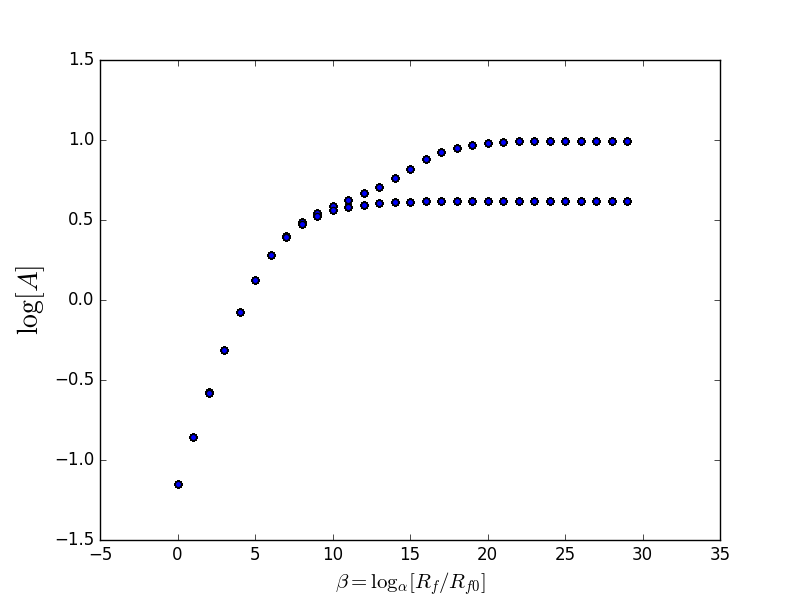
\includegraphics[width=1.0\textwidth]{figure/Lorenz96_single/action.png}
\caption{Lorenz 96 D=10 L=4 action plot for all 100 initial guesses.}
\label{fig:lorenz96}
\end{figure}

\begin{figure}[h]
\centering
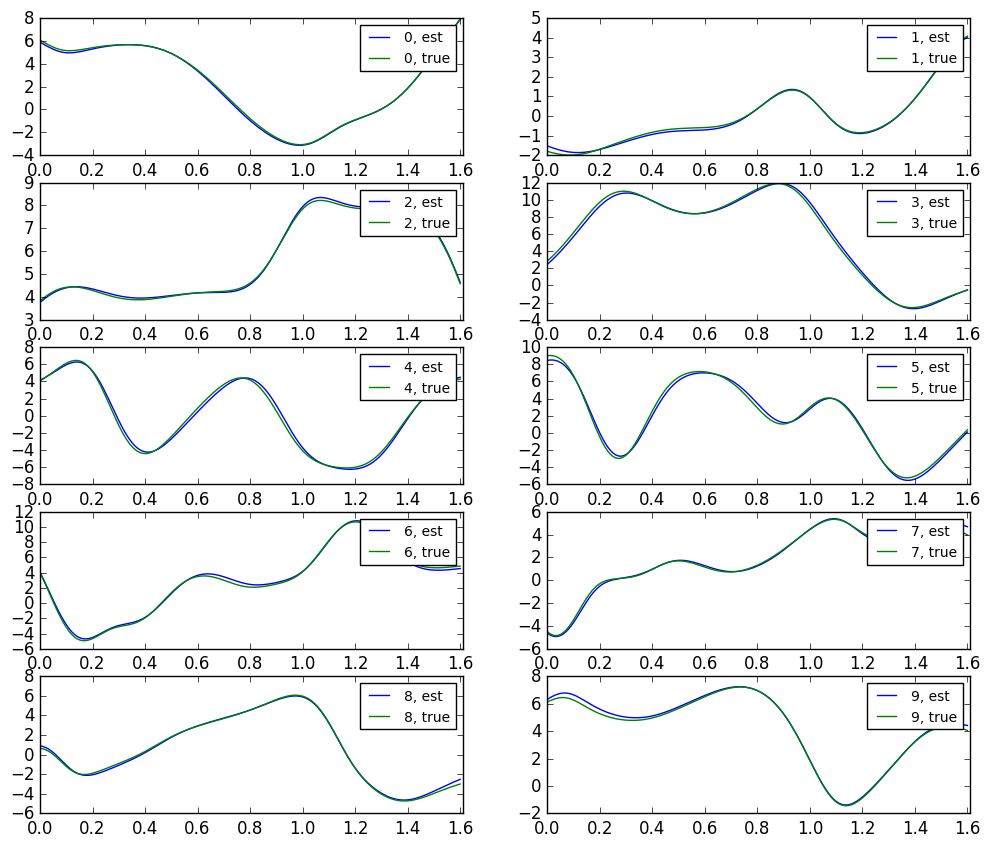
\includegraphics[width=1.0\textwidth]{figure/Lorenz96_single/estimation.png}
\caption{Lorenz 96 D=10 L=4 estimate for lowest action level.}
\end{figure}


\clearpage

%%         L96 multiple data

\subsection{Lorenz96 D=10 (mutiple data sets)}

equations.txt is the same as in the previous section.

\paragraph{\underline{specs.txt}}
\begin{verbatim}
# N/2 (total data is 161 steps, at dt = 0.01)
80
# Skipped data 
100
# Twice the timestep of the data file
0.02
# Input format of files (2: several datasets, no initial condition)
2
# 100 initial conditions for each data set
100
# data files have extension .txt
txt
./observations/observations_
# Stimuli data file paths (none)
# State variable bounds and Rf0 values
-15, 15, 0.01
-15, 15, 0.01
-15, 15, 0.01
-15, 15, 0.01
-15, 15, 0.01
-15, 15, 0.01
-15, 15, 0.01
-15, 15, 0.01
-15, 15, 0.01
-15, 15, 0.01
# Control variable bounds (none)
# Parameter bounds (last line is correct value; not read)
0, 20, 8.17
# Alpha, min beta, max beta
2,1,30
\end{verbatim}

\paragraph{\underline{sub.sh}}

\begin{verbatim}
#!/bin/bash
#$ -t 100-599
#$ -N lorenz96_cpp
#$ -cwd
#$ -j y
#$ -S /bin/bash
#$ -m beas
#$ -o ./output
#$ -e ./error
#$ -q batch.q
./lorenz96_cpp $SGE_TASK_ID
\end{verbatim}


\begin{figure}[h]
\centering
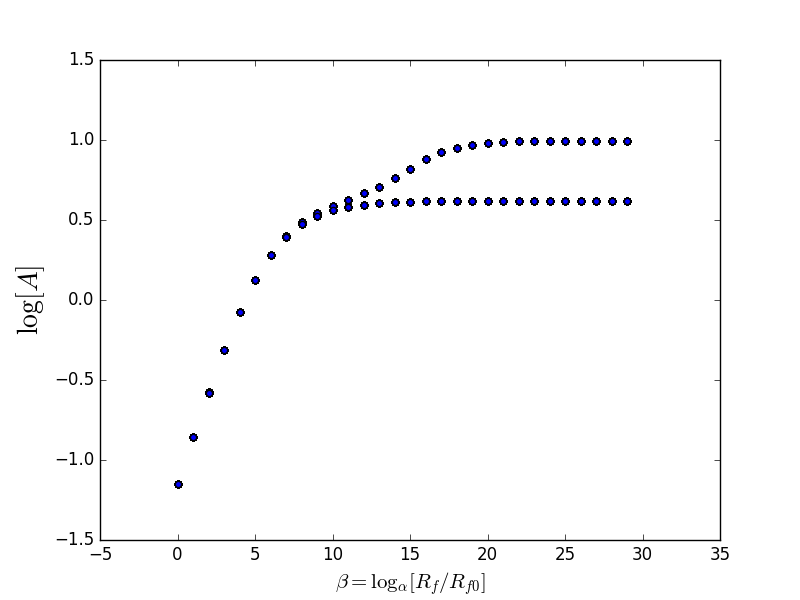
\includegraphics[width=0.47\textwidth]{figure/Lorenz96_multiple/action_path_1.png}
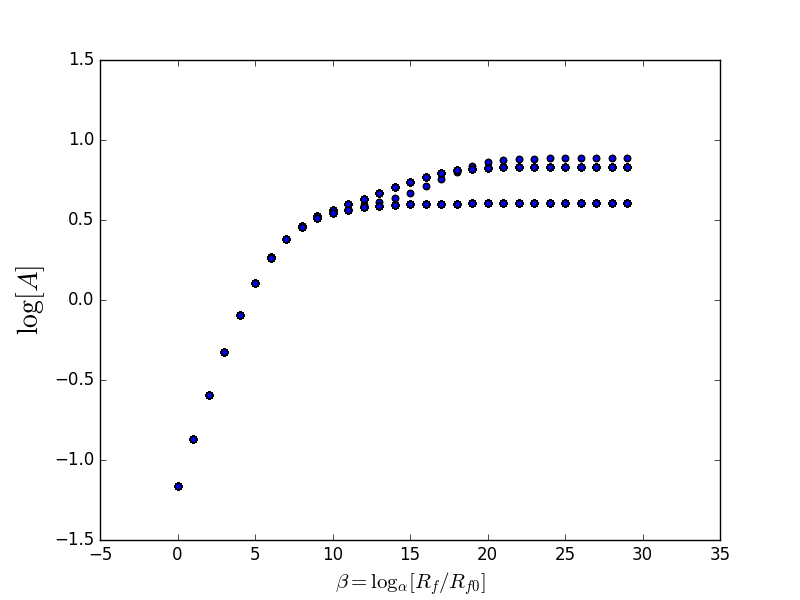
\includegraphics[width=0.47\textwidth]{figure/Lorenz96_multiple/action_path_2.png} \\
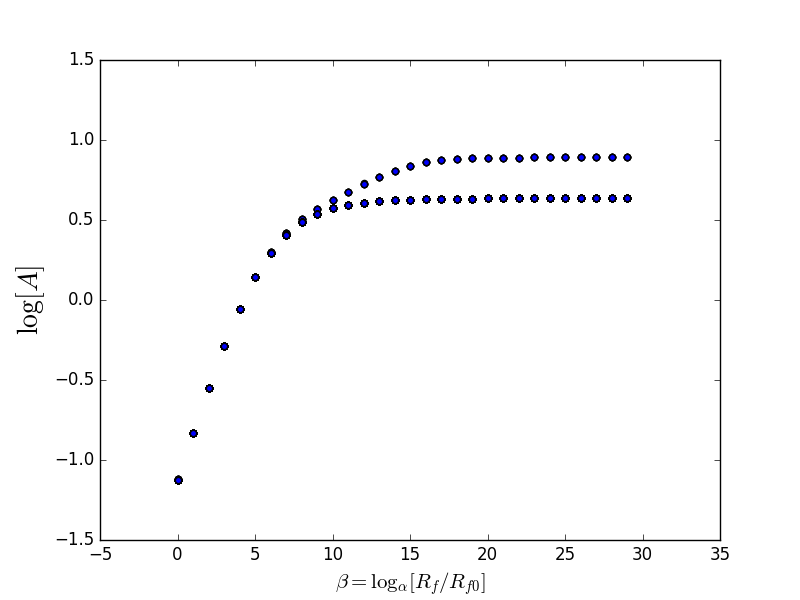
\includegraphics[width=0.47\textwidth]{figure/Lorenz96_multiple/action_path_3.png}
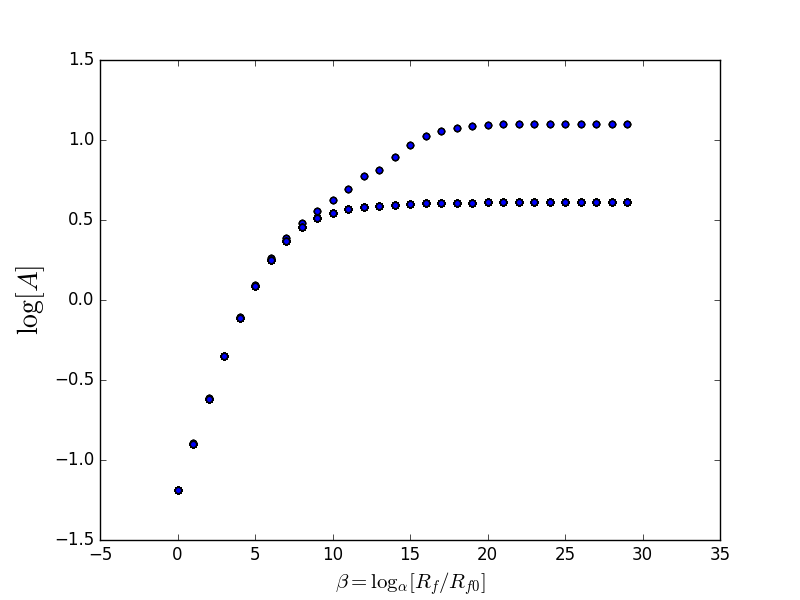
\includegraphics[width=0.47\textwidth]{figure/Lorenz96_multiple/action_path_4.png} \\
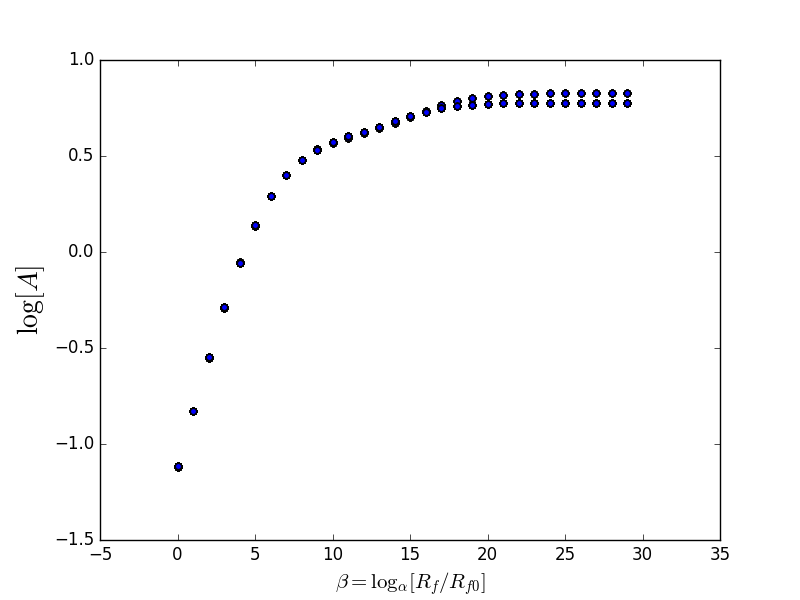
\includegraphics[width=0.47\textwidth]{figure/Lorenz96_multiple/action_path_5.png}
\caption{Lorenz 96 D=10 L=4 action plots for the 5 data sets.}
\label{fig:lorenz96_multiple}
\end{figure}

\begin{figure}[h]
\centering
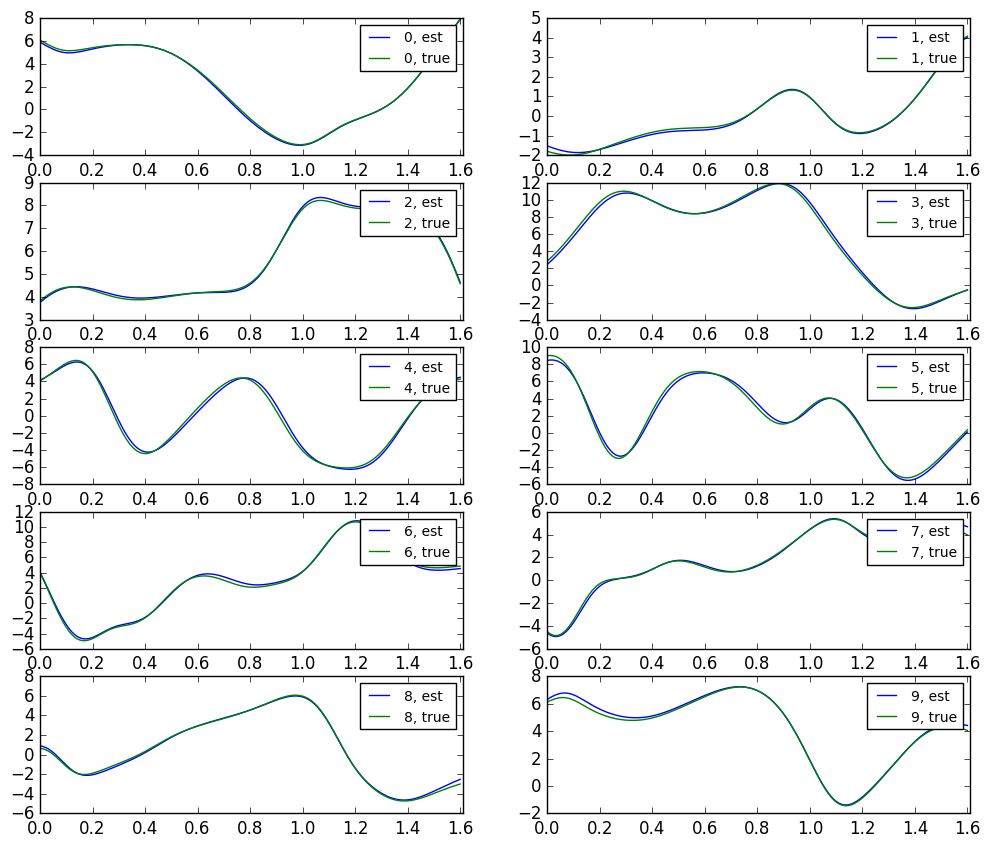
\includegraphics[width=1\textwidth]{figure/Lorenz96_multiple/estimation_1.png} \\
\caption{Lorenz 96 D=10 L=4 estimate for lowest action levels for data set 1. Data set 1 is the same used in the previous example, and one sees that both the action plot and best estimate are identical.}
\end{figure}

\begin{figure}[h]
\centering
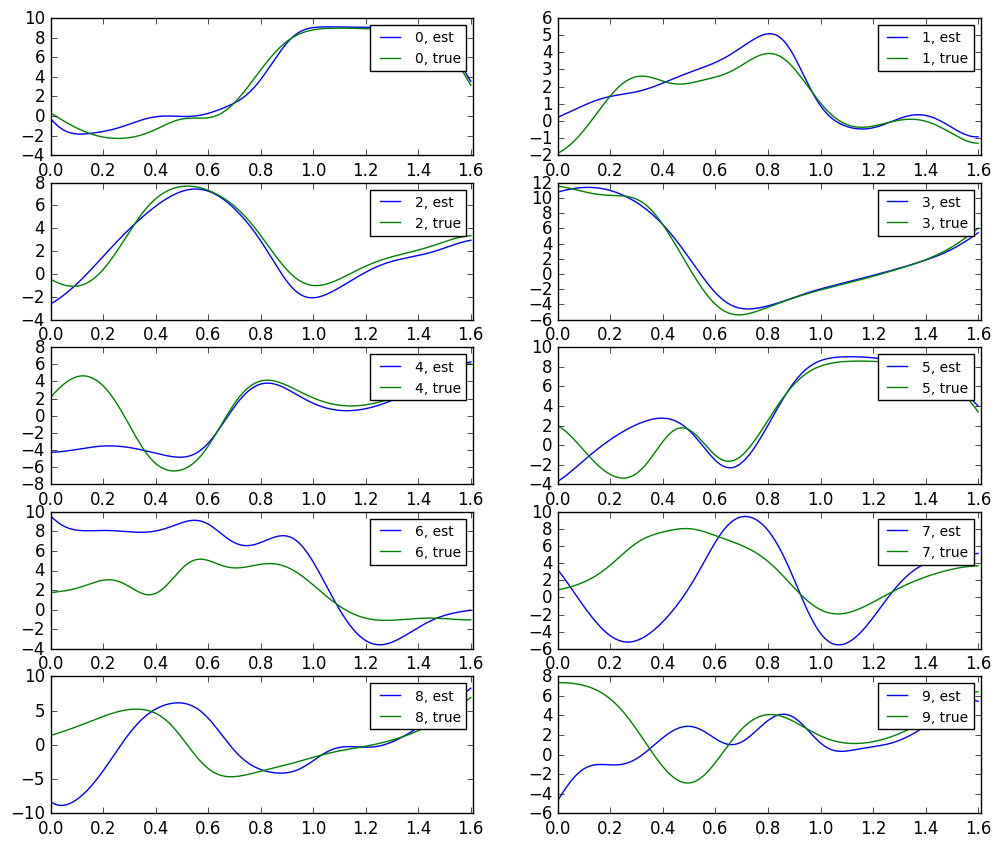
\includegraphics[width=1\textwidth]{figure/Lorenz96_multiple/estimation_5.png} \\
\caption{Lorenz 96 D=10 L=4 estimate for lowest action levels for data set 5. Here the lowest action level gives a poorer estimate. This is consistent with the action plots (Figure \ref{fig:lorenz96_multiple}), where it is seen that the lowest action level for the 5th data set is not quite near the expected value of about 4.}
\end{figure}


\clearpage


%%         L96 synchronizing

\subsection{Lorenz96 D=10 (synchronizing control terms)}

\paragraph{\underline{Vector field}}
\begin{align*}
\frac{dx_1}{dt}&= x_{10}(x_2-x_9)-x_1+f + u_1(y_1 - x_1)\qquad &&\frac{dx_2}{dt}= x_1(x_3-x_{10})-x_2+f + u_2(y_2 - x_2)\\
\frac{dx_3}{dt}&= x_2(x_4-x_1)-x_3+ f + u_3(y_3- x_3) \qquad &&\frac{dx_4}{dt}= x_3(x_5-x_2)-x_4+f+ u_4(y_4 - x_4)\\
\frac{dx_5}{dt}&= x_4(x_6-x_3)-x_5+f \qquad & &\frac{dx_6}{dt}= x_5(x_7-x_4)-x_6+f\\
\frac{dx_7}{dt}&= x_6(x_8-x_5)-x_7+f  \qquad &&\frac{dx_8}{dt}= x_7(x_9-x_6)-x_8+f\\
\frac{dx_9}{dt}&= x_8(x_{10}-x_7)-x_9+f  \qquad  &&\frac{dx_{10}}{dt} = x_9(x_1-x_8)-x_{10}+f
\end{align*}
\paragraph{\underline{equations.txt}}
\begin{verbatim}
# Problem Name
lorenz96
# nY,nP,nU,nI,nF,nM
10,1,3,0,0,3
# Dynamical equations (including synchronization terms)
yy9*(yy1-yy8)-yy0+FF1 + u1*(data0-yy0)
yy0*(yy2-yy9)-yy1+FF1 + u2*(data1-yy1)
yy1*(yy3-yy0)-yy2+FF1 + u3*(data2-yy2)
yy2*(yy4-yy1)-yy3+FF1 
yy3*(yy5-yy2)-yy4+FF1
yy4*(yy6-yy3)-yy5+FF1
yy5*(yy7-yy4)-yy6+FF1
yy6*(yy8-yy5)-yy7+FF1
yy7*(yy9-yy6)-yy8+FF1
yy8*(yy0-yy7)-yy9+FF1
# Measurement terms of cost function 
(data0-yy0)*(data0-yy0) + (data1-yy1)*(data1-yy1) + (data2-yy2)*(data2-yy2) 
+ u1*u1 +u2*u2 + u3*u3
# Variable names
yy0
yy1
yy2
yy3
yy4
yy5
yy6
yy7
yy8
yy9
# Control names
u1
u2
u3
# Parameter names
FF1
# Data names
data0
data1
data2
# Stimuli names (none)
# External functions (none)
\end{verbatim}

\paragraph{\underline{specs.txt}}
\begin{verbatim}
# N/2 (Using 401 data points from data files)
200
# Skipped data 
100
# Twice the timestep of the data file
0.02
# Input format of files (2: data in single file)
2
# (0: there is only 1 dataset, but all measurements in 1 file)
0
txt
observations/observations_1
# Stimuli data file paths (none)
# State variable bounds and Rf0 values (Rf0 high to enforce constraints strictly)
-15, 15, 10^8
-15, 15, 10^8
-15, 15, 10^8
-15, 15, 10^8
-15, 15, 10^8
-15, 15, 10^8
-15, 15, 10^8
-15, 15, 10^8
-15, 15, 10^8
-15, 15, 10^8
# Control variable bounds and initial values
-1,1,1
-1,1,1
-1,1,1
# Parameter bounds (last line is correct value; not read)
0, 20, 8.17
# Alpha, min beta, max beta (only 1 step optimization)
2,1,1
# Output format (2: save control variables to file)
-2
\end{verbatim}

\paragraph{\underline{sub.sh}}
\begin{verbatim}
#!/bin/bash
#$ -t 1-100
#$ -N lorenz96_cpp
#$ -cwd
#$ -j y
#$ -S /bin/bash
#$ -m beas
#$ -o ./output
#$ -e ./error
#$ -q batch.q
./lorenz96_cpp $SGE_TASK_ID
\end{verbatim}

\begin{figure}[h]
\centering
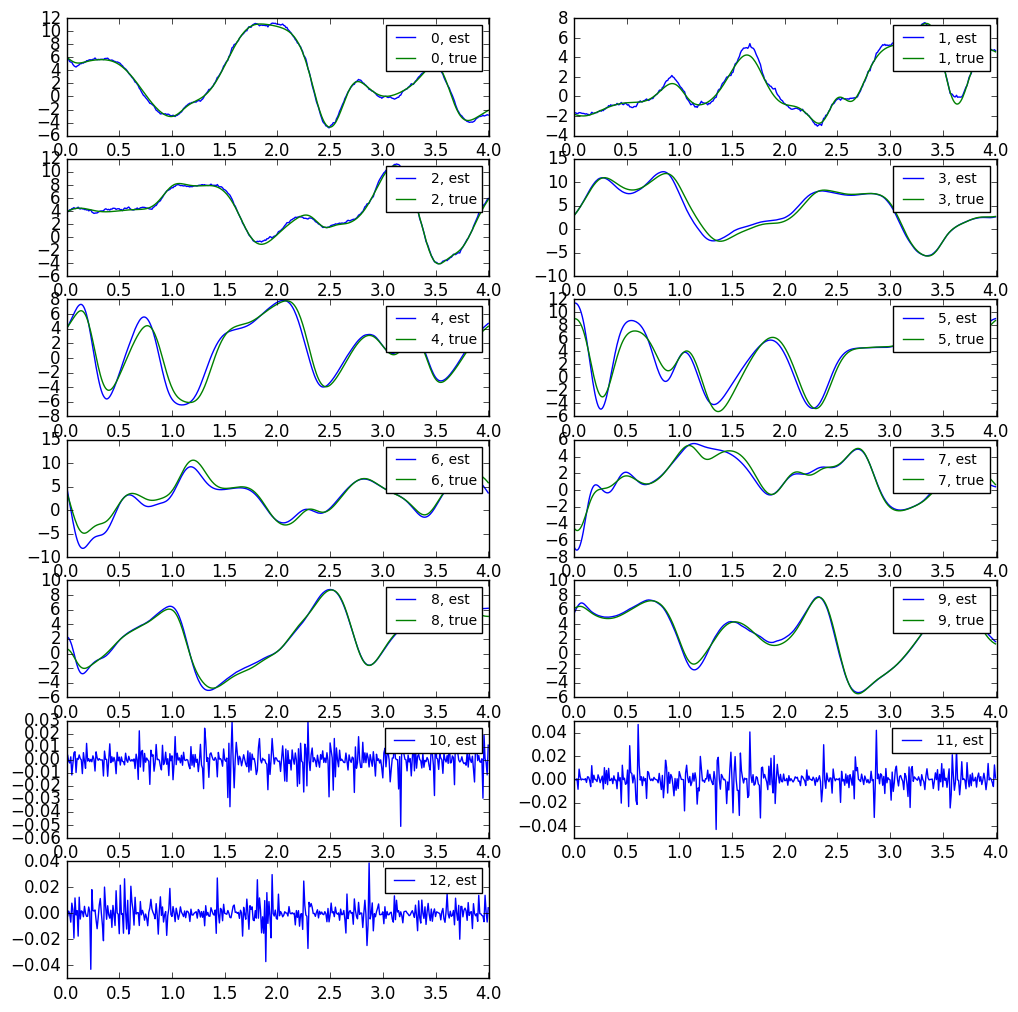
\includegraphics[width=1\textwidth]{figure/Lorenz96_syn/estimation.png} \\
\caption{Lorenz 96 D=10 L=3 estimate for lowest action level. The last three variables are the control terms. The forcing parameter FF1 was estimated to be about 8.149 (true value 8.17).}
\end{figure}

\clearpage

% NAKL

\subsection{NaKL}
\paragraph{Vector field}
\begin{align*}
\frac{dV}{dt}&=CI_{inj}(t) + g_{Na}m^3h(E_{Na}-V) + g_{K}n^4(E_K-V) + g_L(E_L-V)\\
\frac{da}{dt}&=\frac{a_\infty-a}{\tau_a}, ~~~~a=\{m, h, n\}\\
a_\infty&=\frac12+\frac12\tanh\left(\frac{V-V_a}{\Delta V_a}\right)\\
\tau_a&=\tau_{a0}+\tau_{a0}\left(1-\tanh^2\left(\frac{V-V_a}{\Delta V_a}\right)\right)
\end{align*}


\paragraph{\underline{equations.txt}}
\begin{verbatim}
simple_nakl
4,19,0,1,0,1
# Dynamical equations (dV/dt, dn/dt, dh/dt, dm/dt)
gNa*(m0*m0*m0*h0)*(ENa-V0)+gK*n0*n0*n0*n0*(EK-V0)+gL*(EL-V0)+Area*Iinj
(0.5*(1+tanh((V0-Vmo)*dVm)) - m0)/(Cm1+Cm2*(1.0-tanh((V0-Vmo)*dVm)
*tanh((V0-Vmo)*dVm)))
(0.5*(1+tanh((V0-Vho)*dVh)) - h0)/(Ch1+Ch2*(1.0-tanh((V0-Vho)*dVh)
*tanh((V0-Vho)*dVh)))
(0.5*(1+tanh((V0-Vno)*dVn)) - n0)/(Cn1+Cn2*(1.0-tanh((V0-Vno)*dVn)
*tanh((V0-Vno)*dVn)))
# Measurement term of objective function
(VDATA0 - V0)*(VDATA0 - V0)
# State variable names
V0
m0
h0
n0
# Control variable names (none)
# Parameter names
gNa
ENa
gK
EK
gL
EL
Area
Vmo
dVm
Cm1
Cm2
Vho
dVh
Ch1
Ch2
Vno
dVn
Cn1
Cn2
# Data names
VDATA0
# External stimuli names
Iinj
# Externally defined functions (none)
\end{verbatim}

\paragraph{\underline{specs.txt}}

\begin{verbatim}
# N/2 (total data is 6001 steps, at dt = 0.01)
3000
# Skipped data (none)
0
# Twice the timestep of the data file (data taken at 50 kHz)
0.04
# Input format of files (1: single data set, initial condition file)
1
# Initial data file
./input_data/initial_guess.dat
# Measured data file paths (one for each measurement)
./input_data/noise_measured.dat
./input_data/current.dat
# State variable bounds and Rf0 values
-150,70,1e-3
0, 1,1e1
0, 1,1e1
0, 1,1e1
# Control variable bounds (none)
# Parameter bounds (plus true values and names, which aren't read)
50,200,120, gNa
0,100,50, ENa
5,40,20, gK
-100,-50,-77, EK
0.1,1,.3, gL
-60,-50,-54, EL
0.5,1.5,0.8, Area
-60,-30,-40, Vmo
.01,0.1,0.06667, dVm
0.05,.25,.1, Cm1
.1,1,.4, Cm2
-70,-40,-60, Vho
-0.1,-.01,-.06667, dVh
.1,5,1, Ch1
1,15,7, Ch2
-70,-40,-55, Vno
.01,0.1,.03333, dVn
.1,5,1, Cn1
2,12,5, Cn2
# Anneal settings
2,1,30
\end{verbatim}

\paragraph{\underline{sub.sh}}

\begin{verbatim}
#!/bin/bash
#$ -t 1-100
#$ -N simple_nakl_cpp
#$ -cwd
#$ -j y
#$ -S /bin/bash
#$ -m beas
#$ -o ./output
#$ -e ./error
#$ -q batch.q
./simple_nakl_cpp $SGE_TASK_ID
\end{verbatim}

\begin{figure}[h]
\centering
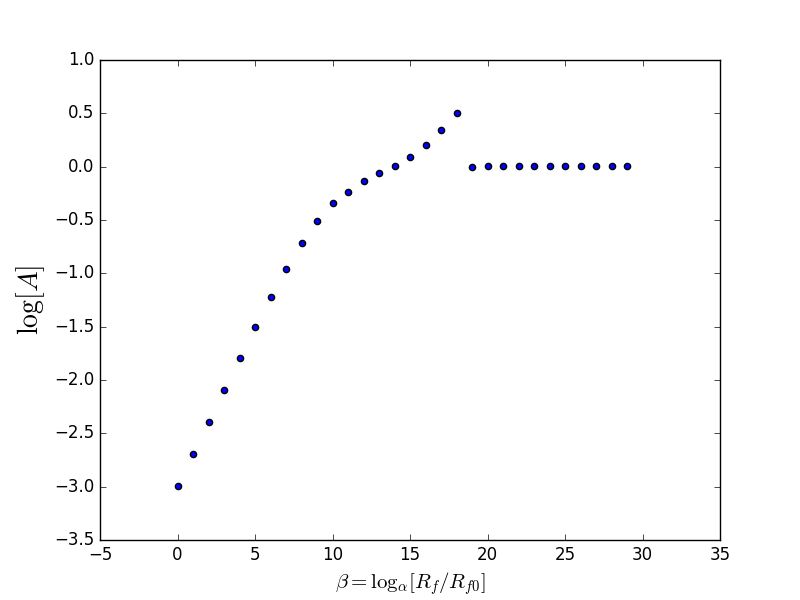
\includegraphics[width=1\textwidth]{figure/NaKL/action.png}
\caption{NaKL model action plot.}
\label{fig:NaKL}
\end{figure}

\begin{figure}[h]
\centering
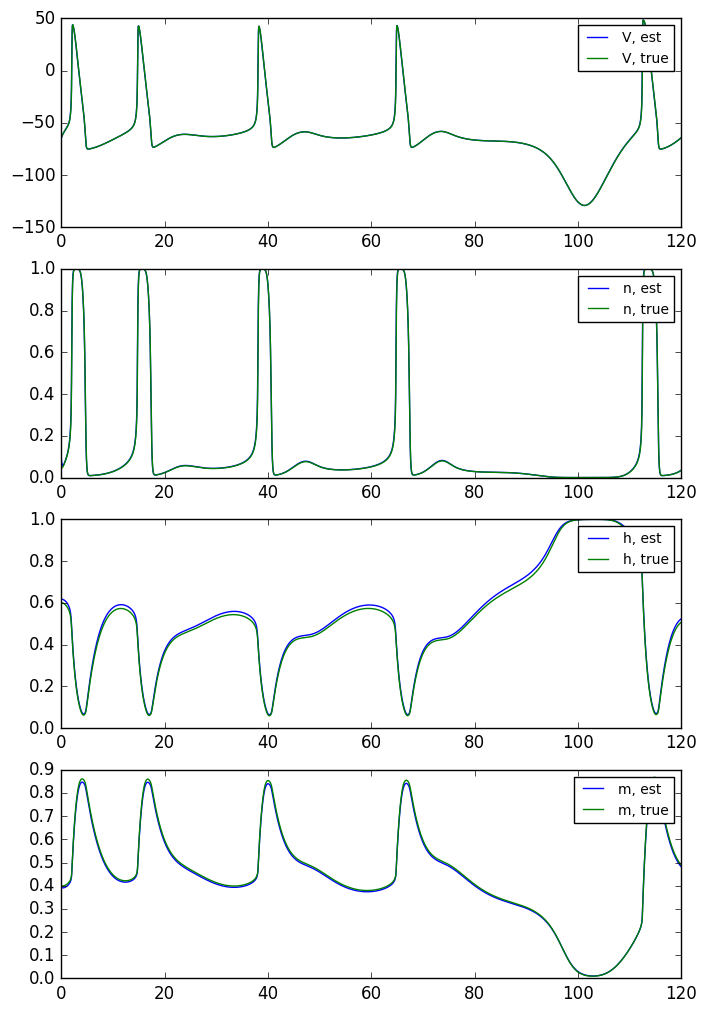
\includegraphics[width=0.8\textwidth]{figure/NaKL/estimation.png}
\caption{NaKL model best estimate, compared against the true trajectories.}
\label{fig:NaKL}
\end{figure}



\clearpage



% L96 External Functions

\subsection{Lorenz96 D = 10 (externally-defined functions)}


\paragraph{\underline{equations.txt}}
\begin{verbatim}
lorenz96
# nY,nP,nU,nI,nF,nM
10,1,0,0,1,5
# Dynamical equations (including synchronization terms)
Lorenzvectorfield(yy0,yy1,yy9,yy8,FF1)
Lorenzvectorfield(yy1,yy2,yy0,yy9,FF1)
Lorenzvectorfield(yy2,yy3,yy1,yy0,FF1)
Lorenzvectorfield(yy3,yy4,yy2,yy1,FF1)
Lorenzvectorfield(yy4,yy5,yy3,yy2,FF1)
Lorenzvectorfield(yy5,yy6,yy4,yy3,FF1)
Lorenzvectorfield(yy6,yy7,yy5,yy4,FF1)
Lorenzvectorfield(yy7,yy8,yy6,yy5,FF1)
Lorenzvectorfield(yy8,yy9,yy7,yy6,FF1)
Lorenzvectorfield(yy9,yy0,yy8,yy7,FF1)
# Measurement terms of cost function 
(data0-yy0)*(data0-yy0) + (data1-yy1)*(data1-yy1) + (data2-yy2)*(data2-yy2) 
+ (data3-yy3)*(data3-yy3) + (data4-yy4)*(data4-yy4)
# Variable names
yy0
yy1
yy2
yy3
yy4
yy5
yy6
yy7
yy8
yy9
# Control names (none)
# Parameter names
FF1
# Data names
data0
data1
data2
data3
data4
# Stimuli names (none)
# External functions (defined in myfunctions.hpp file)
Lorenzvectorfield, 5
\end{verbatim}

\paragraph{\underline{specs.txt}}

\begin{verbatim}
# N/2
200
# Skipped data 
100
# Twice the timestep of the data file
0.02
# Input format of files (2: data in single file)
2
# (0: there is only 1 dataset, but all measurements in 1 file)
0
txt
observations/observations_1
# Stimuli data file paths (none)
# State variable bounds and Rf0 values
-15, 15, 0.0001
-15, 15, 0.0001
-15, 15, 0.0001
-15, 15, 0.0001
-15, 15, 0.0001
-15, 15, 0.0001
-15, 15, 0.0001
-15, 15, 0.0001
-15, 15, 0.0001
-15, 15, 0.0001
# Control variable bounds and initial values (none)
# Parameter bounds (last line is correct value; not read)
0, 20, 8.17
# Alpha, min beta, max beta 
2,1,30
\end{verbatim}

\paragraph{\underline{sub.sh}}

\begin{verbatim}
#!/bin/bash
#$ -t 1-100
#$ -N lorenz96_cpp
#$ -cwd
#$ -j y
#$ -S /bin/bash
#$ -m beas
#$ -o ./output
#$ -e ./error
#$ -q batch.q
./lorenz96_cpp $SGE_TASK_ID
\end{verbatim}

\subsubsection{External function definitions in myfunctions.hpp}

The \texttt{myfunctions.hpp} file includes definitions of the user-defined functions that were declared in \texttt{equations.txt}. This header file has 3 functions: the function itself, its gradient function, and its Hessian matrix. The name of the function itself must align with that declared in \texttt{equations.txt}. Likewise, the name of the gradient function must be the function name with ``jac'' appended at the end, while the Hessian function must be the same string plus ``hes.'' Also, the variables in the argument list of each function must be in the same order as they are called whenever the function is evoked in \texttt{equations.txt}. Note that the argument list can contain parameters or dynamical states alike. 

The gradient function contains an extra argument ``n'', which is the value of the variable with which the derivative is being taken with respect to: the acceptable values start at 1 (this means the derivative with respect to the first variable in the argument list). The gradient function should returned a different value for each ``n,'' depending on the functions derivative with respect to that particular variable.

The Hessian functions in the same way, now with two argument ``n'' and ``m,'', denoting the variable with respect to which the derivative is taken first, and then second, respectively. 


\paragraph{\underline{myfunctions.hpp}}


\begin{verbatim}
#include <cmath>
#include <cstdlib>
#include <iostream>
#include <fstream>

using namespace std;

double Lorenzvectorfield(double x, double x_p1, double x_m1, 
                          double x_m2, double forcing)
{
  // Lorenz model equations; x = x_n, x_m1 = x_(n-1), 
  // x_m2 = x_(n-2), x_p1 = x_(n+1)
  double value=0.0;
  value = x_m1*(x_p1-x_m2) - x + forcing;
  return value;
}

double Lorenzvectorfieldjac(double x, double x_p1, double x_m1, 
                             double x_m2, double forcing, int n)
{
  double value=0.0;
  switch (n) {
    case 1:
    // derivative with respect to x
      value = -1; break;
    case 2:
    // derivative with respect to x_p1
      value = x_m1; break;
    case 3:
    // derivative with respect to x_m1
      value = x_p1 - x_m2; break;
    case 4:
    // derivative with respect to x_m2
      value = -x_m1; break;
    case 5:
    // derivative with respect to forcing
      value = 1; break;
    default:
      cout << "Error in user-defined function jacobian";break;
  } // end switch
  return value;
}

double Lorenzvectorfieldhes(double x, double x_p1, double x_m1, 
                     double x_m2, double forcing, int n, int m)
{
  double value=0.0;
  switch (n) {
    case 1:
    // derivative with respect to x
      value = 0; break;
    case 2:
    // derivative with respect to x_p1
      if (m == 3){
         value = 1; break;
      }
      else{
         value = 0; break;
      }      
    case 3:
    // derivative with respect to x_m1
        if (m == 2){
           value = 1; break;
        }
        else if (m == 4){
           value = -1; break;
        }      
        else{
           value = 0; break;
        }      
    case 4:
    // derivative with respect to x_m2
        if (m == 3){
           value = -1; break;
        }
        else{
           value = 0; break;
        }      
    case 5:
    // derivative with respect to forcing
      value = 0; break;
    default:
      cout << "Error in user-defined function Hessian";break;
  } 
  return value;
}
\end{verbatim}


\begin{figure}[h]
\centering
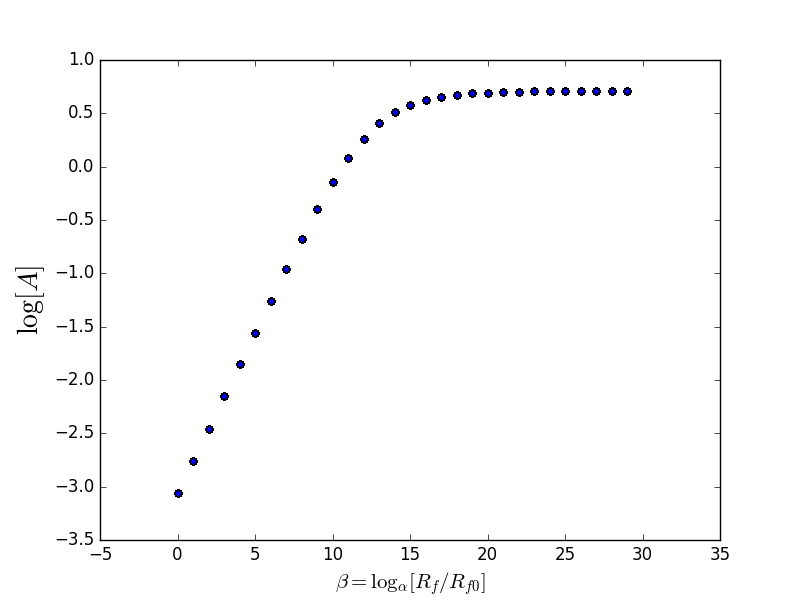
\includegraphics[width=.8\textwidth]{figure/Lorenz96_ext/action.png}
\caption{Lorenz96 model action plot, with $L = 5$. The results here will be identical if the functions (here externally-defined) were insteadinput explicitly in \texttt{equations.txt}.}
\label{fig:Lorenz96_ext_action}
\end{figure}

\begin{figure}[h]
\centering
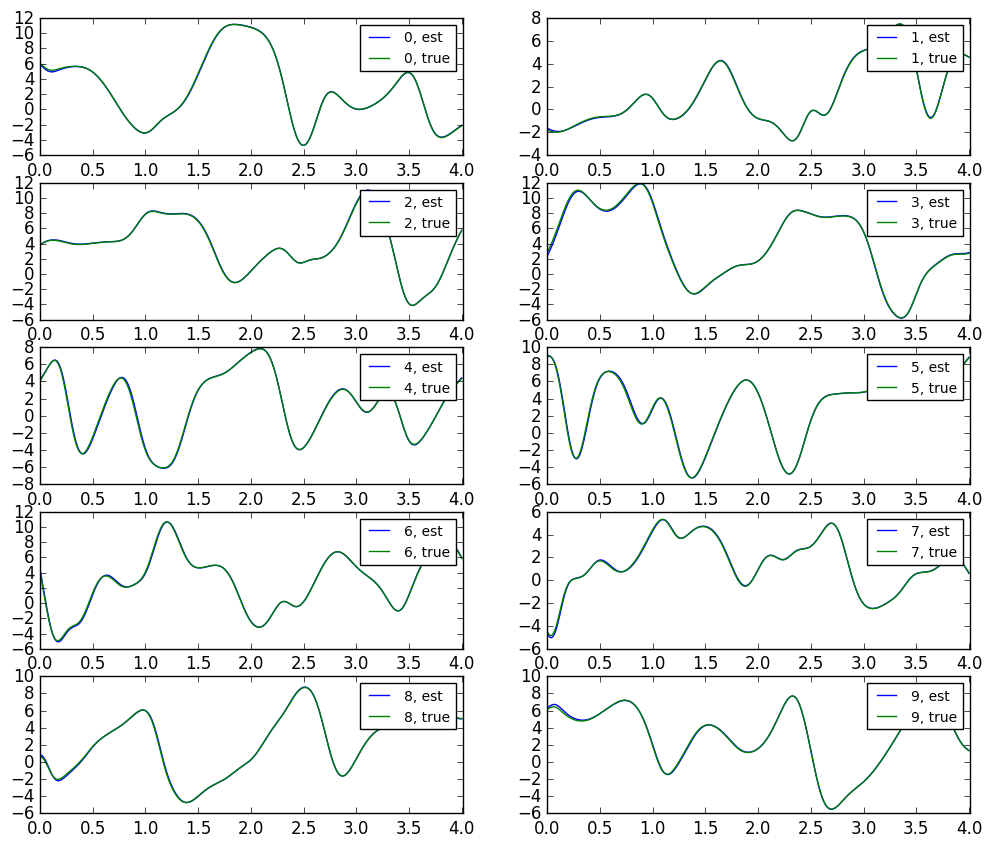
\includegraphics[width=1\textwidth]{figure/Lorenz96_ext/estimation.png}
\caption{Lorenz96 model estimated trajectories. Five variables is sufficient to give excellent estimations for all 100 runs of the annealing.}
\label{fig:Lorenz96_ext_path}
\end{figure}


\clearpage


%% this section deleted
\iffalse
\newpage
\section{New Features}
\subsection{ Resubmission Feature (added 2015/4/9)}
\subsubsection{Description}
For some historical reason, it is complicated to configure data files to start the annealing process with a bunch of given initial paths. However, when the annealing method is applied to some large scale dynamical systems like complex neuron model and neural networks, it is often killed by job manager system after its running time exceeds 24 hours. The target of this update is to allow one can continue the computation starting with old path data files obtained from previous annealing calculation conveniently.
\subsubsection{Installation}
If you are using the old version \texttt{minAone} right now, you can simply replace the old \texttt{minAone.py} with the new one. Done!!!
\subsubsection{Data File Configuration}
Current version only reads the data files named by \texttt{D\%d\_M\%d\_PATH\%d.dat} located in the same directory with executive file. After you change initial condition indicator to be 1 in \texttt{specs.txt}, and add another dummy filename after that line, the $i$th annealing process will look for the last line of \texttt{D\%d\_M\%d\_PATH}$i$\texttt{.dat}. Note the path data are arranged in the following way
\begin{verbatim}
beta exitflag action_value 
optimal_path[x1(0) x2(0) x3(0) x4(0) x5(0)  x1(1) x2(1) x3(1) 
x4(1) x5(1) ... x1(NT) x2(NT) x3(NT) x4(NT) x5(NT)
 p(1) p(2) ... p(NP)]
\end{verbatim}
$\beta$ value is initialed by the first integer of the line plus beta step increment, exitflag and action value will be omitted automatically, and then the initial path is filled by the remaining numbers of the line.

If the file \texttt{D\%d\_M\%d\_PATH}$i$\texttt{.dat} is not found, its initial path will be generated with random numbers. The program doesn't check completeness of the path file, and the code seeks the last path line by line, so please make sure your path data file \texttt{D\%d\_M\%d\_PATH}$i$\texttt{.dat} has a complete path in EACH line(not only the last line).

In summary, the following is the list of the steps
\begin{enumerate}
\item change initial condition indicator to be 1 in \texttt{specs.txt}, and add another {\color{red}dummy} filename after that line. 
\item put all the \texttt{D\%d\_M\%d\_PATH\%d.dat} files in the same directory with the executive file, make sure the numbers after letter \texttt{D} and letter \texttt{M} in the filename are consistent with the information in your \texttt{equations.txt}
\item run the executive file
\end{enumerate}
\paragraph{Warning:} The resubmission feature would introduce round-off errors. Double precision data are outputted into the file in the format of \texttt{\%e}, when those data are read back into the code, it may introduce round-off errors. In the example of Lorenz96, the round-off error caused the final optimal values of the cost function differed from regular calculation values by $0\sim25$.
\fi

%%% End of deleted section

\section{Troubleshooting}
I have tested these scripts over a wide range of problems, so I believe that the algorithms are correct. However, there are a few common errors that may crop up.
\begin{itemize}
\item Variable and parameter naming is very important. Never use a variable name that includes the name of another variable. For instance p1 and p11 would be bad, since p11 includes p1. In this case, p01 and p11 would be adequate. Along this vein, all variable names should be at least 2 characters long, just in case. The external functions name should not contain any numbers or other characters -- only letters.
\end{itemize}
\end{document}
